\documentclass[aspectratio=169]{beamer}
\usepackage{will_handley_beamer}
\usepackage{title_page}
\usepackage{listings}
\usepackage{xcolor}

\definecolor{codegreen}{rgb}{0,0.6,0}
\definecolor{codegray}{rgb}{0.5,0.5,0.5}
\definecolor{codepurple}{rgb}{0.58,0,0.82}
\definecolor{backcolour}{rgb}{0.95,0.95,0.92}

\lstdefinestyle{mystyle}{
    backgroundcolor=\color{white},   
    commentstyle=\color{C2},
    keywordstyle=\color{C3},
    numberstyle=\tiny\color{C0},
    stringstyle=\color{C1},
    basicstyle=\ttfamily\tiny,
	identifierstyle=\color{black},
    breakatwhitespace=false,         
    breaklines=true,                 
    captionpos=b,                    
    keepspaces=true,                 
    numbers=left,                    
    numbersep=5pt,                  
    showspaces=false,                
    showstringspaces=false,
    showtabs=false,                  
    tabsize=2
}

\lstset{style=mystyle}


% Commands
% --------
% - \arxiv{arxiv number}
% - \cols{width}{lh column}{rh column}
% -  \begin{fig(left|right)}[fractional width (e.g 0.6) ]{name of image}
%        content of other column
%    \end{fig(left|right)}

% Talk details
% ------------
\title{ScannerBit 2.0}
\subtitle{Sampling techniques in high-dimensional parameter spaces}
\date{23\textsuperscript{rd} Feb 2024}

\begin{document}

\begin{frame}
    \titlepage
\end{frame}

\begin{frame}
    \frametitle{What do I mean by parameter spaces?}
\end{frame}

\begin{frame}
    \frametitle{Cosmology \& Astrophysics}
    \begin{columns}
        \column{0.3\textwidth}
        
        \column{0.35\textwidth}
        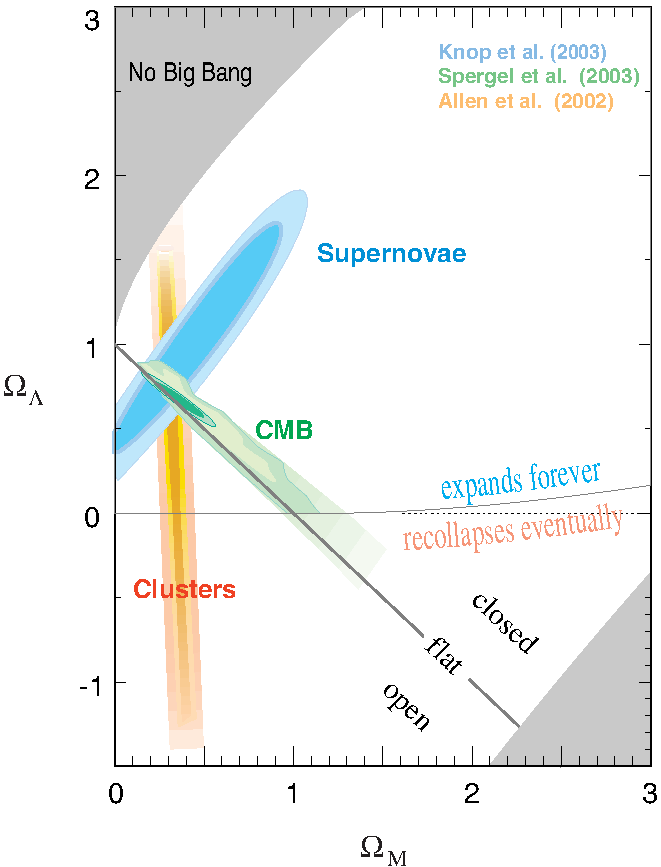
\includegraphics[width=\textwidth]{figures/old_parameters}
        \column{0.25\textwidth}
        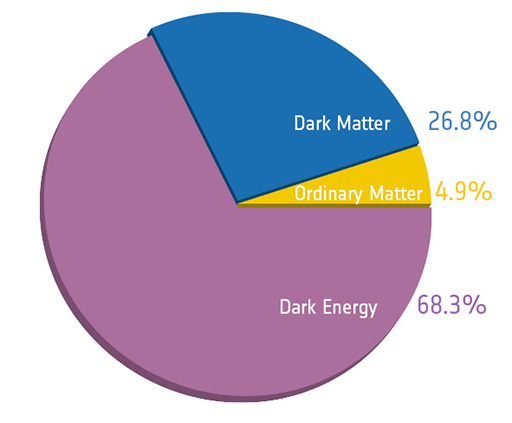
\includegraphics[width=\textwidth]{figures/darkmatterchart_squared}
        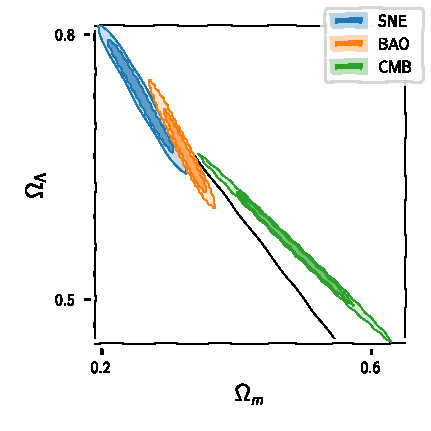
\includegraphics[width=\textwidth]{figures/universe_constraints_zoom}
    \end{columns}

    
\end{frame}

\begin{frame}
    \frametitle{Particle physics}
    \begin{columns}
        \column{0.5\textwidth}
        
        
        \column{0.5\textwidth}
        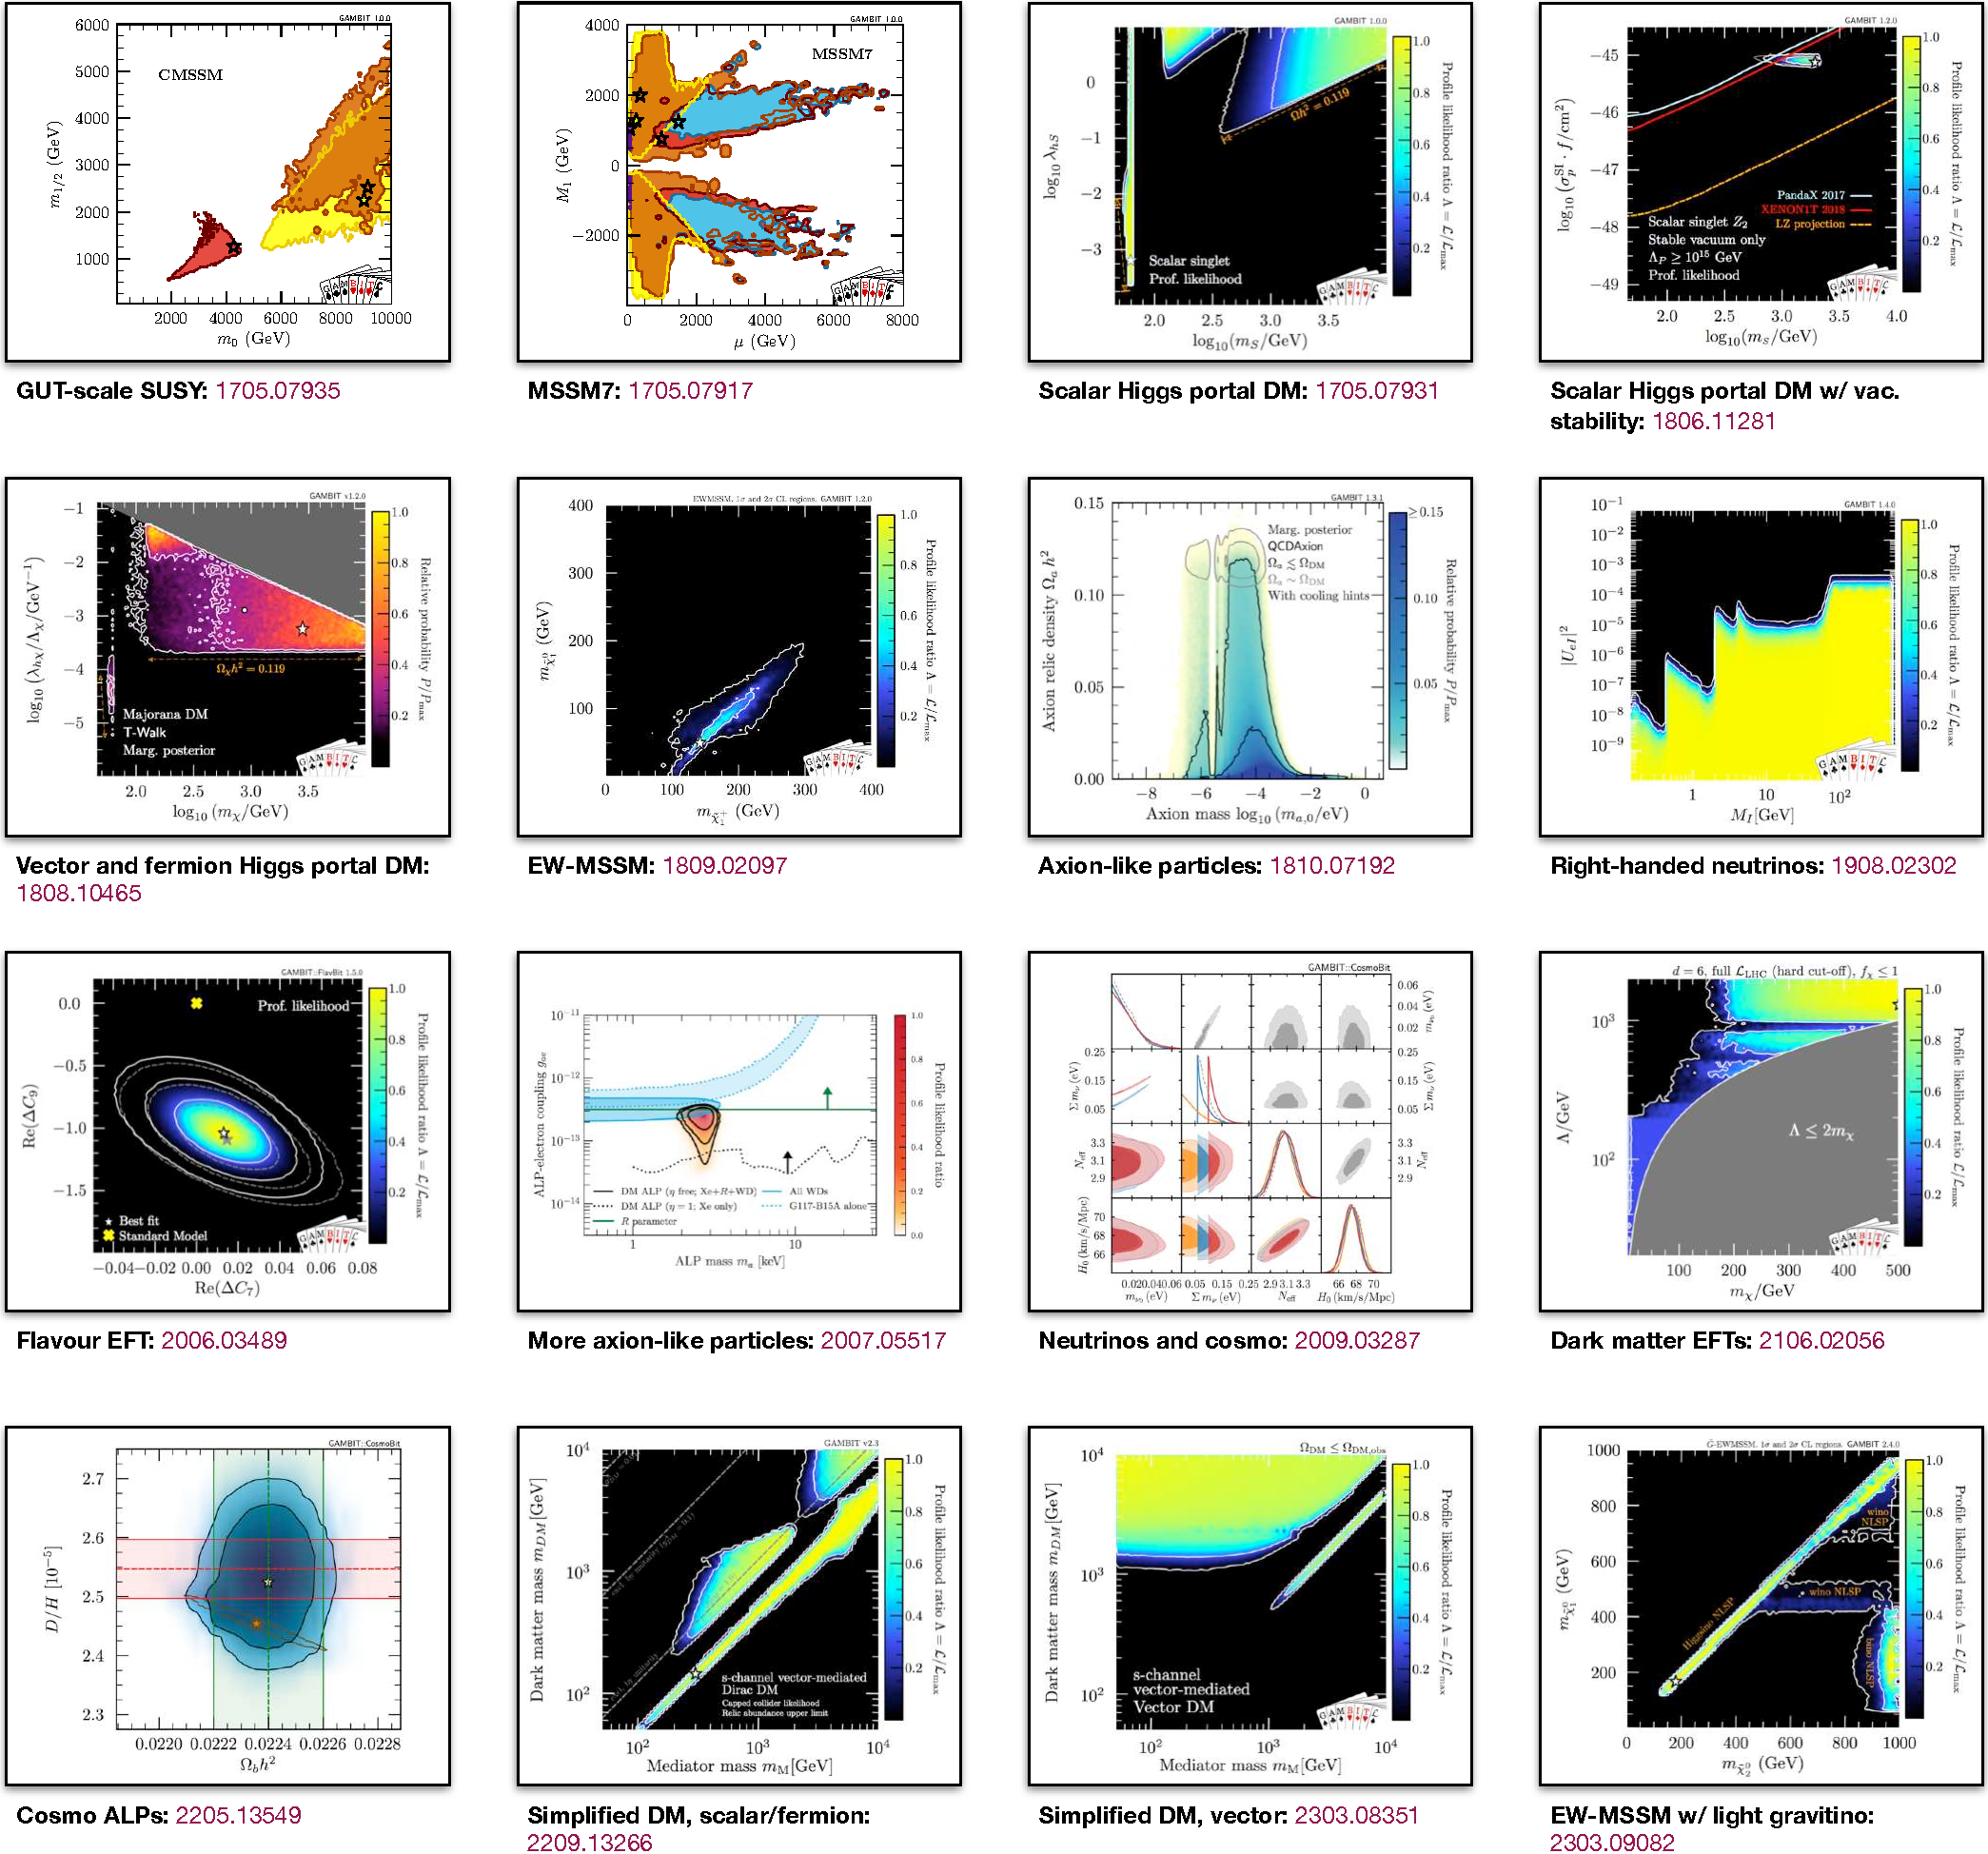
\includegraphics[width=\textwidth]{figures/gambit_examples}
    \end{columns}
    
\end{frame}

\begin{frame}
    \frametitle{Materials/Chemistry}
    \begin{columns}
        \column{0.5\textwidth}
        
        \column{0.35\textwidth}
        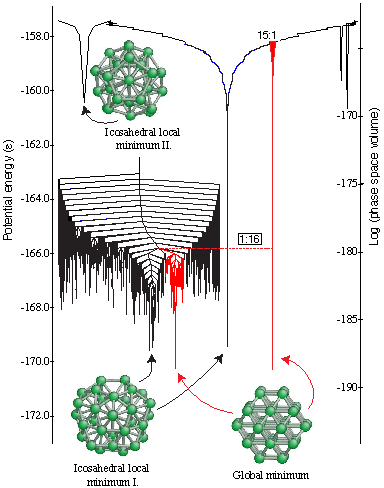
\includegraphics[width=\textwidth]{figures/materials}
        
    \end{columns}
\end{frame}

\begin{frame}
    \frametitle{Biophysics}
    \begin{columns}
        \column{0.5\textwidth}
        
        \column{0.5\textwidth}
        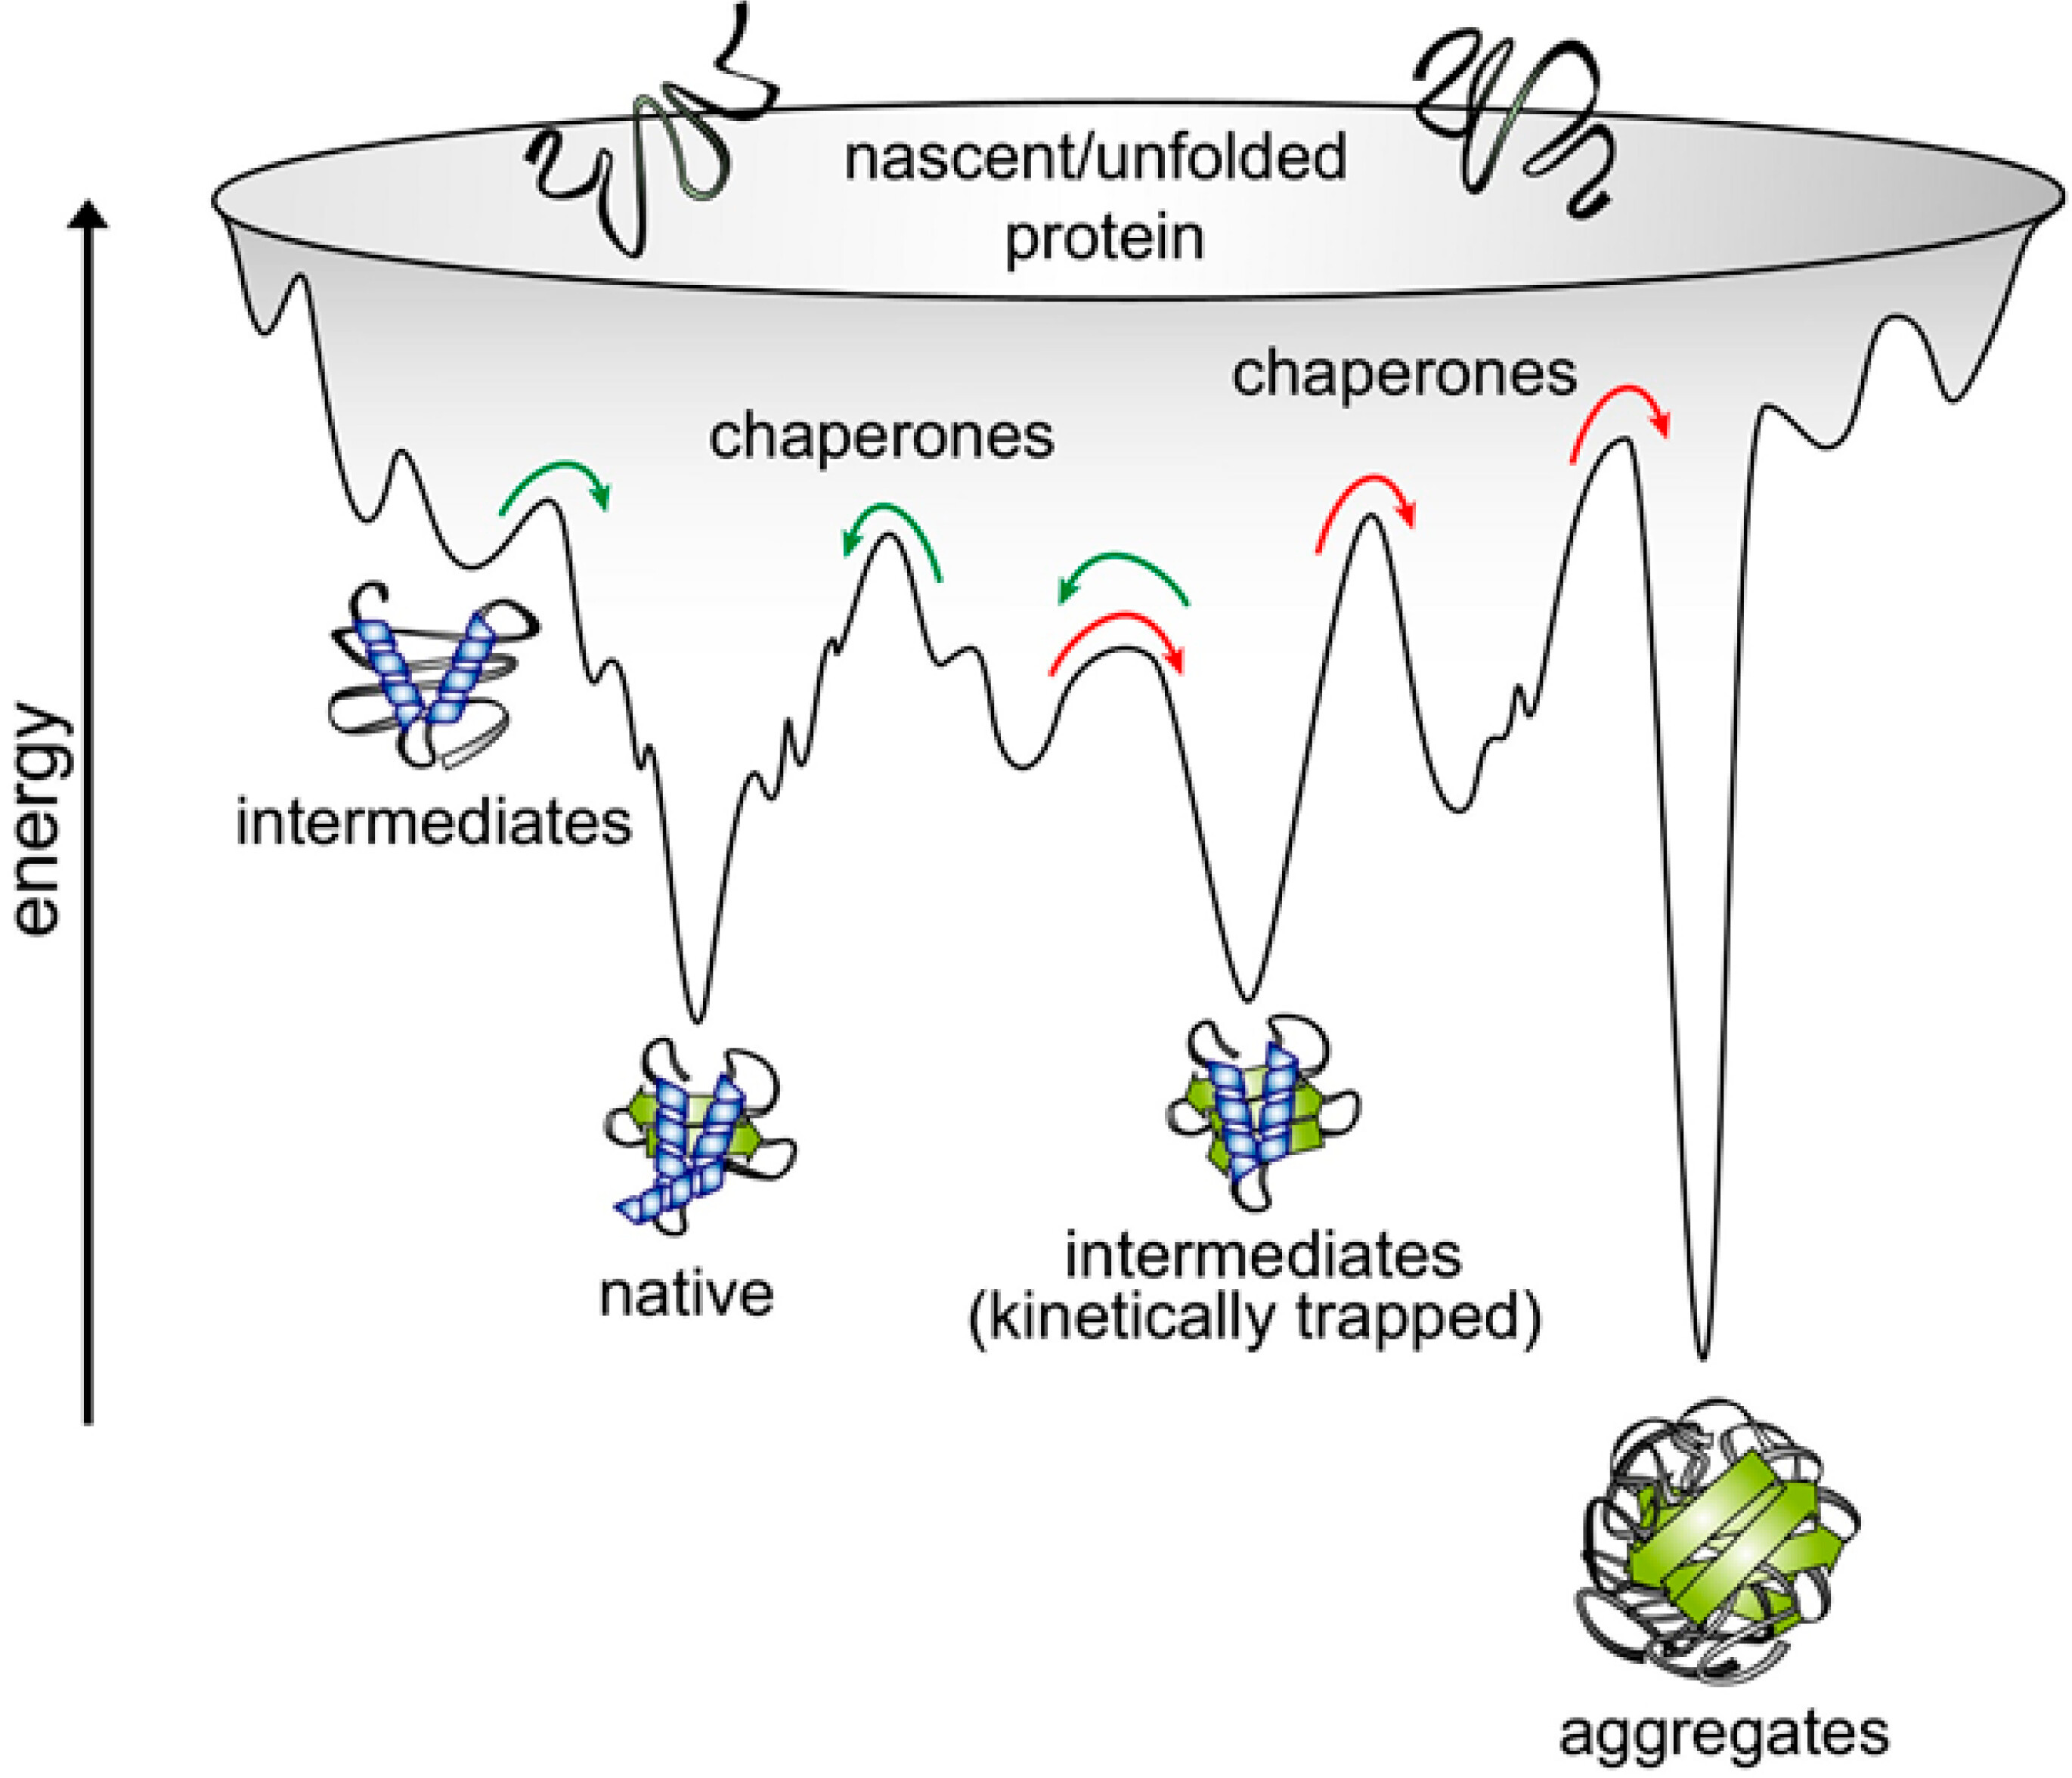
\includegraphics[width=\textwidth]{figures/proteins}
        
    \end{columns}
\end{frame}



\begin{frame}
    \frametitle{Machine learning}
    \begin{columns}
        \column{0.5\textwidth}
        \begin{itemize}
            \item Standard machine learning training setup:
                \[ \hat{\theta} = \min_\theta L(\theta) \]
                \[ L(\theta) = \min_{\theta} \sum_{i\in\text{train}} |f(x_i;\theta)-y_i|^2 \]
                \begin{itemize}
                    \item $x$: input data
                    \item $y$: target data
                    \item $f$: neural network
                    \item $\theta$: model parameters (weights and biases)
                \end{itemize}
            \item The ``Loss function'' $L$, viewed as a function of the model (e.g.\ neural network) parameters $\theta$, is a complicated, high-dimensional surface
        \end{itemize}
        
        \column{0.5\textwidth}
        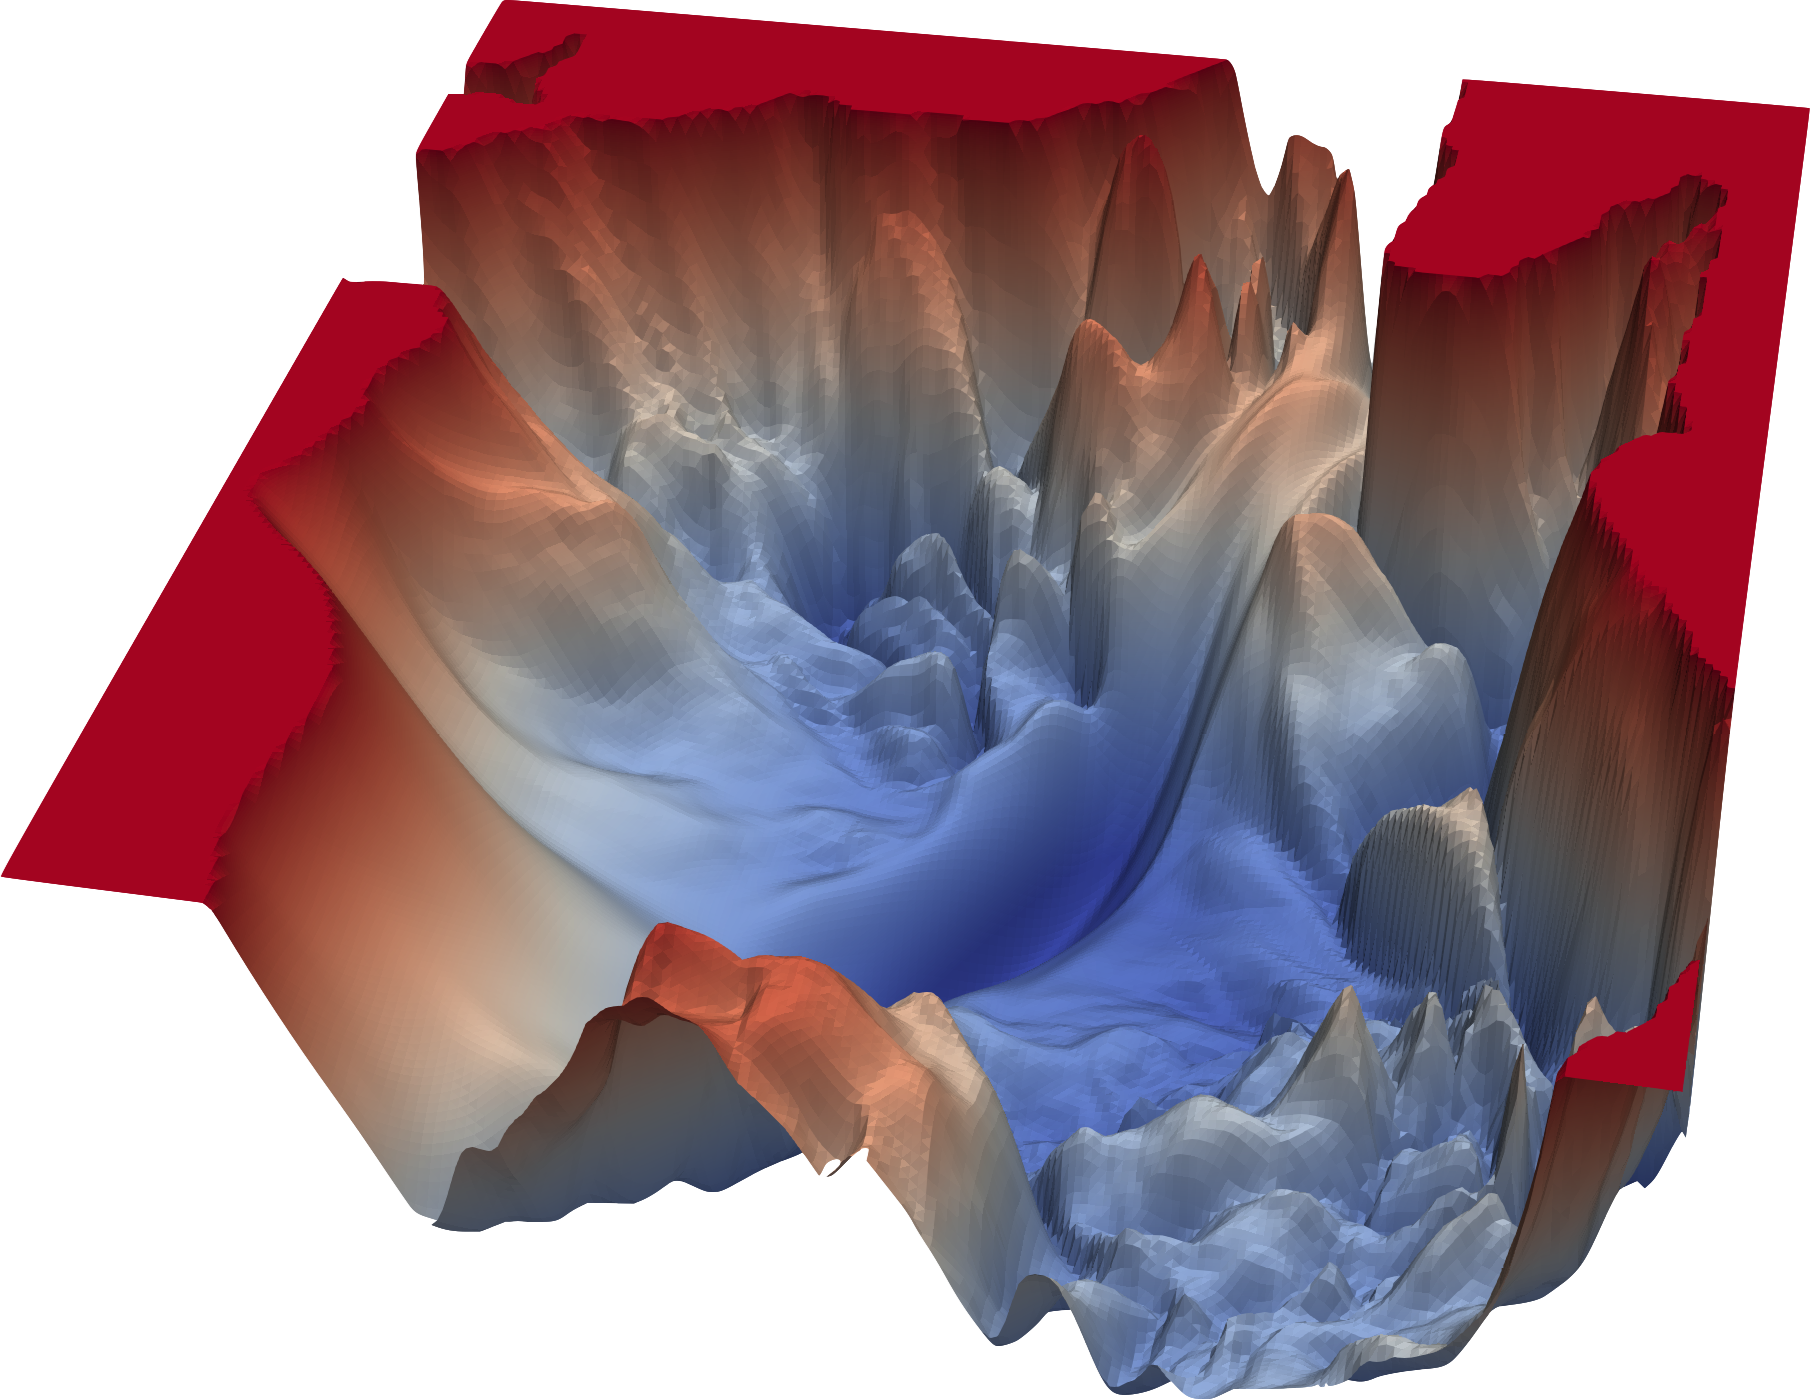
\includegraphics[width=\textwidth]{figures/loss_landscape}

        \hfill\href{https://losslandscape.com}{losslandscape.com}
    \end{columns}
\end{frame}

\begin{frame}
    \frametitle{Exploring parameter spaces}
    Profiling vs Marginalising

    Visualisation requires a 2D projection

    2D has very specific properties which do not lend themselves well to intuiting the behaviour of the full parameter space

    Volumes in high dimensions
    
\end{frame}

\begin{frame}
    \frametitle{Random scanning: how not to do it}
    
\end{frame}

\begin{frame}
    \frametitle{Gradient descent}
\end{frame}

\begin{frame}
    \frametitle{Exploration \& sampling}
\end{frame}

\begin{frame}
    \frametitle{Nested sampling}
\end{frame}

\begin{frame}
    \frametitle{Differential evolution/Genetic Algorithms}
    
\end{frame}

{
    \usebackgroundtemplate{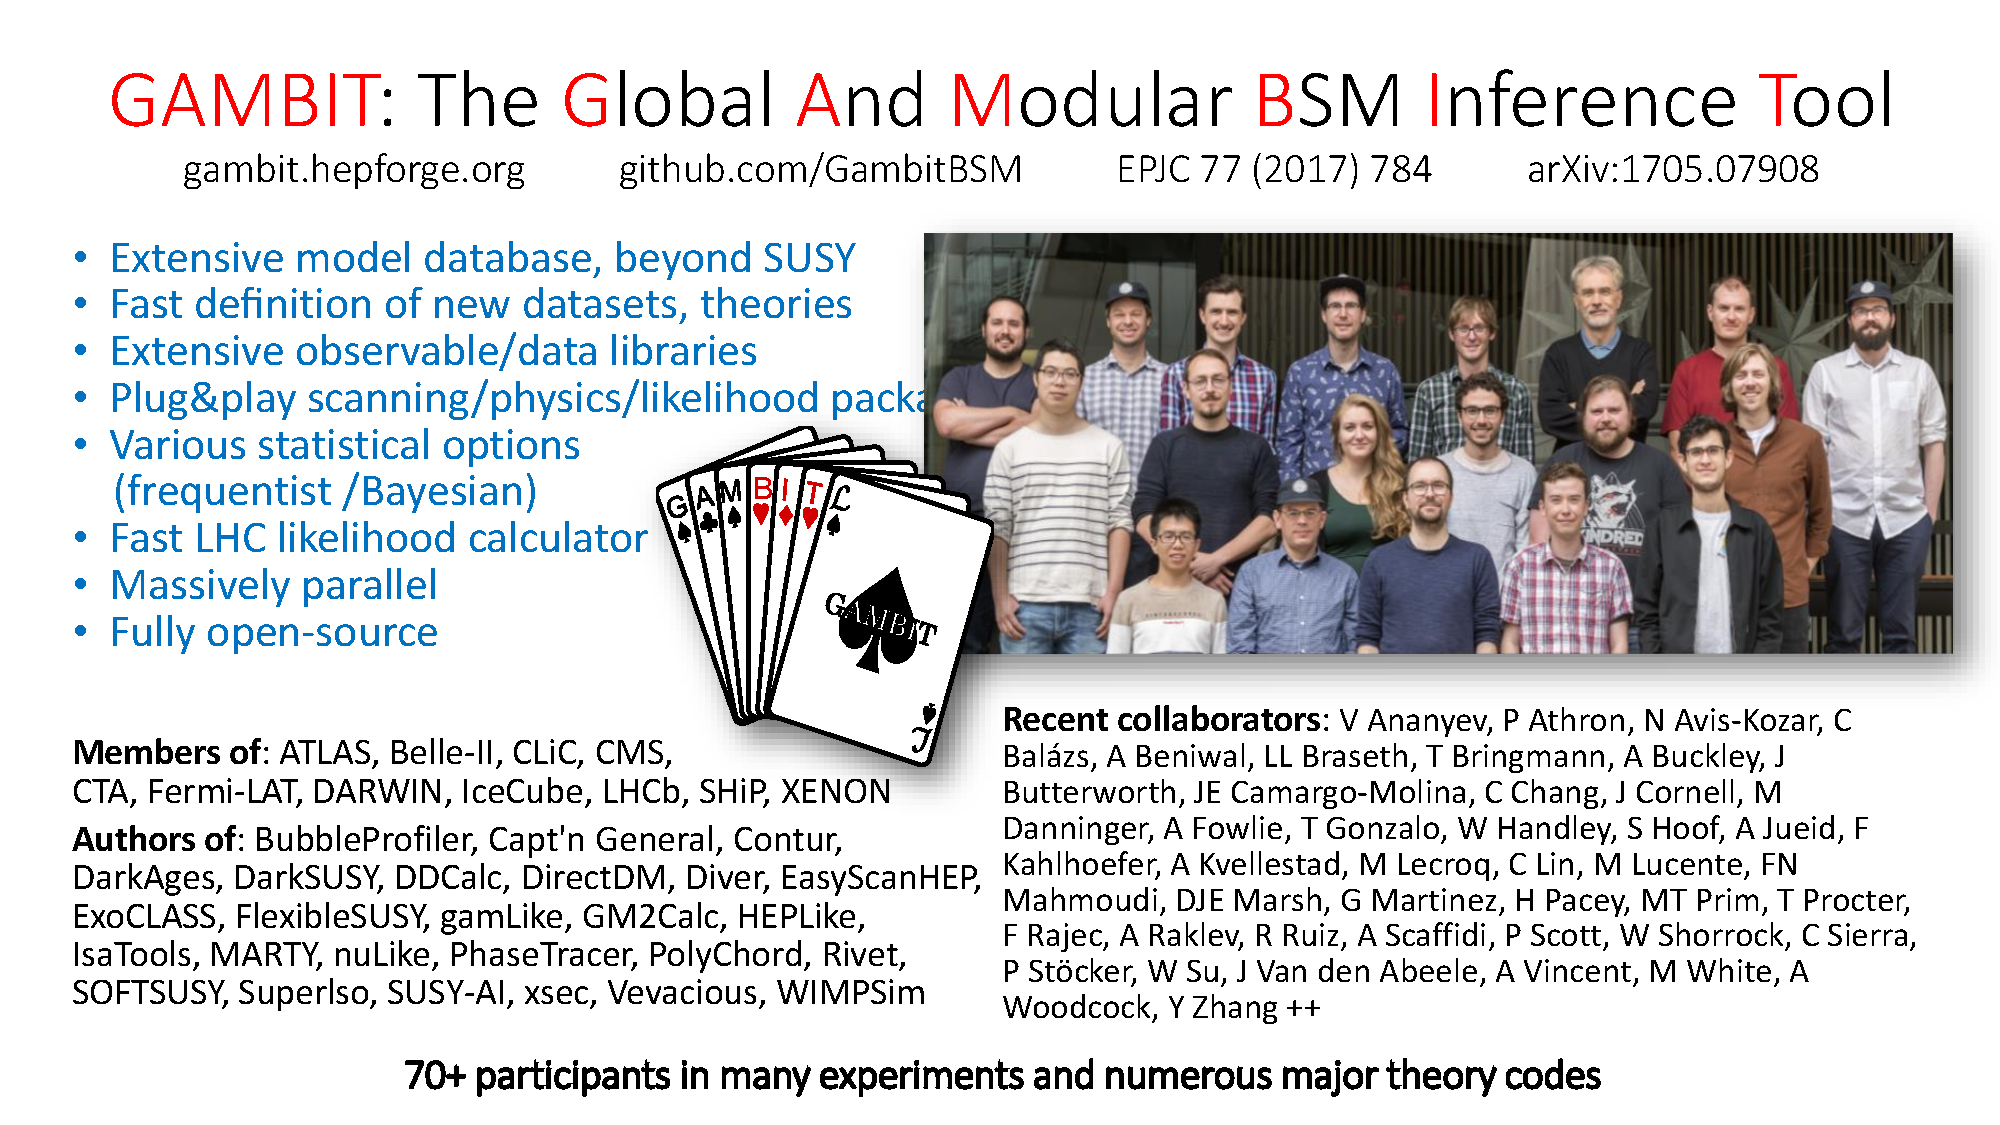
\includegraphics[width=\paperwidth]{gambit_ad_slide}}
    \begin{frame}[plain]
    \end{frame}
}

\begin{frame}
    \frametitle{What is GAMBIT?}
    \begin{columns}
        \column{0.48\textwidth}
        \begin{block}{GAMBIT as a software framework}
            \begin{itemize}
                \item Combines collider, direct detection, neutrino \& telescope data
                \item Allows joint analysis of dark matter, neutrinos \& BSM physics
            \end{itemize}
        \end{block}
        \column{0.48\textwidth}
        \begin{block}{GAMBIT as a community}
            \begin{itemize}
                \item Particle physicists, cosmologists \& statisticians
                \item Generates interdisciplinary expertise \& inspires new techniques
                    %GAMBIT is a framework for combining data from multiple experiments to constrain particle physics and cosmology models. It is both is an open source software framework and a community of high energy physicists, cosmologists and statisticians; capable of linking theory, data and inference approaches allowing the combination of high-energy colliders, direct detection, neutrino experiments and measurements from telescopes using both frequentist and Bayesian paradigms. The power of this set of tools and expertise allows novel analyses of dark matter, neutrinos and beyond the standard model physics which is challenging to achieve with separated datasets.

%This talk will describe GAMBIT, present physics results and map out the prospects for extension.  It will also serve to highlight the key events in the week which people new to the community may wish to come along to, including introductory sessions for installing and using the software.
            \end{itemize}
        \end{block}
    \end{columns}
%    Anders:
%    Highlight when we develop GAMBIT we have HPC systems in mind,
    % two-level paralellisation (MPI to porallelise scanners, openMP to parallelise likelihood computations)
    % recently set a new internal record for utilising the highest number of cores 115,000 CPUs
    % 1000 MPI with 100 threads per MPI
%    Don't expect GAMBIT to be 'pip install gambit'
%    power tool for heavy tasks
%    comes with complications
%
%    Pointing out the modularity of gambit
    % reason why it has grown as a large community is that the code & teams are designed to be modular
    % possible for large groups of people to work in parallel
    % would be more difficult if it were hard-coded
    %
    % UPCOMING:
    % GAMBITLite
    % ScannerBit 2.0
    % 
    % community: don't have *just* long author papers to improve modularity


%Greg
    %design for interface with different types of software (different libraries and languages, python, mathematica FORTRAN C++
    %
    % previous software: cosmomc/superbayes/montepython/coboya/cosmosis
    %plug-and-play with modularity
    % combat ``why don't we just use ultranest/dynesty for everything''

    % Andrew:
    % Community: access to really big computing resources (on average for last 5y have had 40MCPUh/y)
    % - hard to win/have access to on your own
    % 
% More slides
% https://www.dropbox.com/s/2c7c475t6traj42/Data_at_UiO_2022_Kvellestad.pdf?dl=0

%Anders:
    % talk to atlas susy group
    % trivial point which landed well: if we're going to use a smart sampling algorithm, then parallelisation will be non-trivial
    % atlas recently released pmssm, completely random sampling, so they can do sampling, and then parallelised physics computations in increasing levels of complexity offline after the sampling
    % adaptive sampling algorithms _require_ all likelihood computations on the fly.
    % at the end of the day they just classify points as excluded or not
    % https://ui.adsabs.harvard.edu/abs/2022AAS...24030220M/abstract
    % https://www.overleaf.com/9325782714mghdvzmzxtpt#ba83d1
    
\end{frame}

\begin{frame}
    \frametitle{GAMBIT}
    \begin{columns}
        \column{0.4\textwidth}
        \column{0.6\textwidth}
        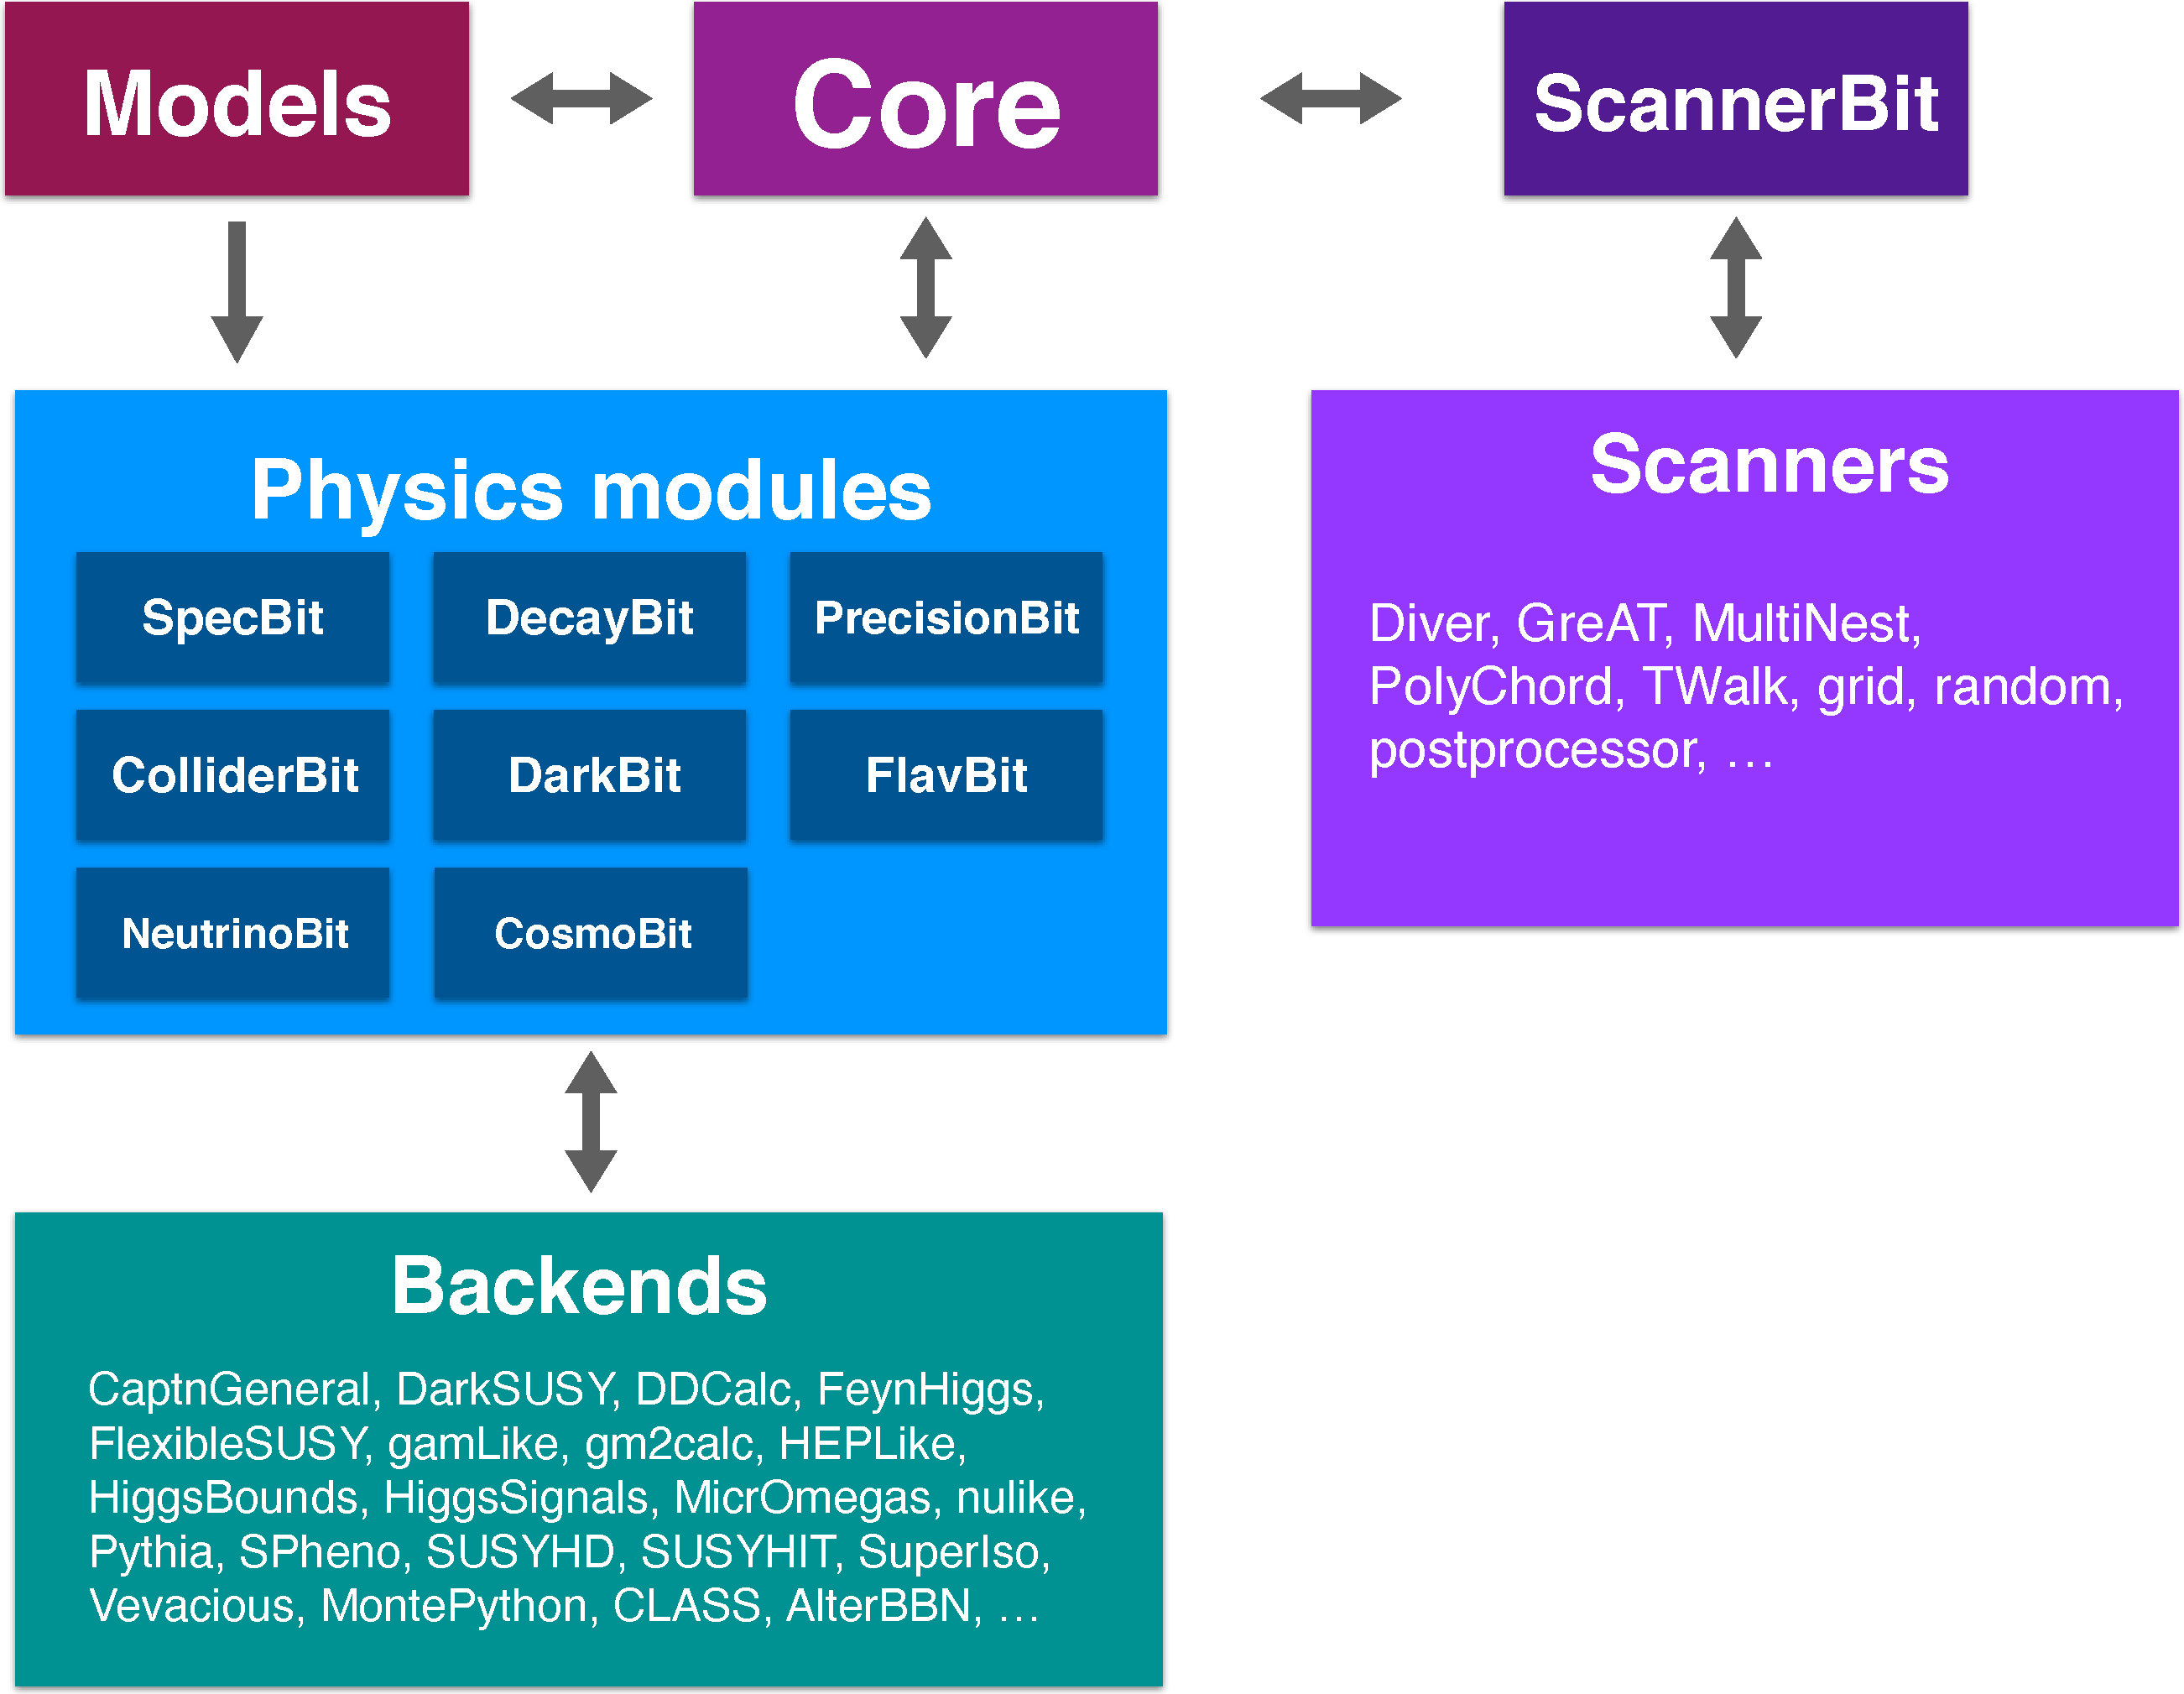
\includegraphics[width=\textwidth]{figures/gambit_layout}
    \end{columns}
\end{frame}

\begin{frame}
    \frametitle{ScannerBit~\arxiv{1705.07959}}
    \begin{columns}
        \column{0.5\textwidth}
        Original paper:
        \begin{itemize}
            \item describes code design \& structure
            \item compares performance of the main two scanning algorithms: \texttt{diver} \& \texttt{MultiNest} 
        \end{itemize}
        %took one model and used several different scanners 15D MSSM scalar singlet (2+13)
        
        \column{0.5\textwidth}
        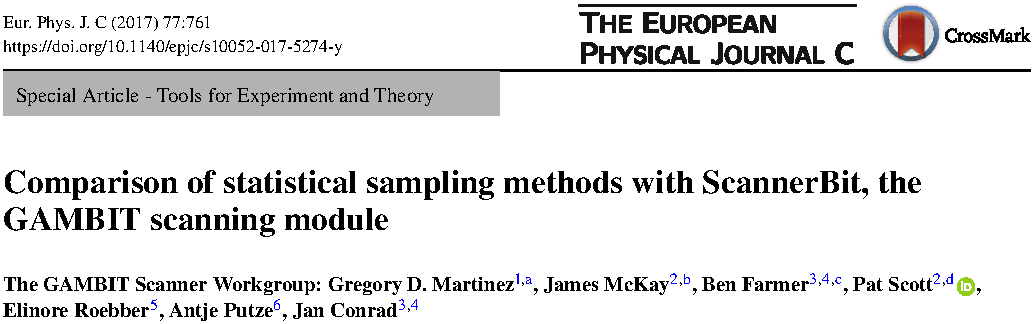
\includegraphics[width=\textwidth]{figures/scannerbit_header}
        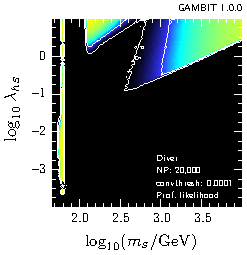
\includegraphics[width=0.5\textwidth]{figures/scannerbit_15d_diver_profile}%
        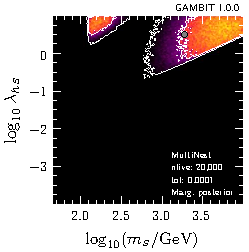
\includegraphics[width=0.5\textwidth]{figures/scannerbit_15d_mn_posterior}
    \end{columns}
\end{frame}

\begin{frame}
    \frametitle{ScannerBit 2.0}
    \begin{columns}
        \column{0.5\textwidth}
        Developments since original ScannerBit paper:
        \begin{enumerate}
            \item New scanning algorithms
                \begin{itemize}
                    \item \texttt{MINUIT2}
                    \item \texttt{PolyChord}
                    \item particle swarm
                \end{itemize}
            \item \texttt{PyScannerBit}
                \begin{itemize}
                    \item Isolation of scanning algorithms from GAMBIT
                    \item documentation: \href{https://pyscannerbit.readthedocs.io}{pyscannerbit.readthedocs.io}
                \end{itemize}
            \item Python Scanners
                \begin{itemize}
                    \item Allows easy incorporation of new scanning algorithms into GAMBIT
                    \item Including modern machine learning techniques
                \end{itemize}
        \end{enumerate}
        \column{0.5\textwidth}
        
    \end{columns}
\end{frame}


\begin{frame}[fragile]
    \frametitle{Python Scanners}
    \begin{columns}
        \column{0.5\textwidth}
        
        \column{0.5\textwidth}
\begin{lstlisting}[language=Python]
"""scipy.optimize scanner."""
import scanner_plugin as splug
import scipy.optimize
import numpy as np


class Minimize(splug.scanner):
    __version__ = scipy_version

    def __init__(self, **kwargs):
        super().__init__(use_mpi=False,
                         use_resume=False)

    def run(self):
        start = np.random.rand(self.dim)
        bounds = [(0., 1.)] * self.dim

        def neg_loglike_hypercube(x):
            return -self.loglike_hypercube(x)

        res = scipy.optimize.minimize(
                  neg_loglike_hypercube,
                  start, bounds=bounds)

        return 0

__plugins__ = {"scipy_minimize": Minimize}
\end{lstlisting}
    \end{columns}
\end{frame}


\begin{frame}[fragile]
    \frametitle{Python Scanners}
    \begin{columns}
        \column{0.5\textwidth}
        
        \column{0.5\textwidth}
\begin{lstlisting}[language=Python]
"""Grid scanner with MPI."""
import scanner_plugin as splug
from utils import MPI
import numpy as np

class Grid(splug.scanner):

    __version__="1.0.0"

    def __init__(self, grid_pts=10, parameters=[],
                 **kwargs):
        super().__init__(use_mpi=True, use_resume=False)
        # Set up grid
        for param in self.parameter_names:
            n = grid_pts[parameters.index(param)]
            self.vecs.append(np.linspace(0.0, 1.0, n))
    
    def run(self):
        # Loop over grid with MPI
        grid = np.meshgrid(*self.vecs)
        grid = grid.reshape(self.dim, -1).T
        grid = grid[self.mpi_rank:self.size:
                    self.mpi_size]
        for pt in grid:
            self.loglike_hypercube(pt)
        return 0

__plugins__={"python_grid": Grid}
\end{lstlisting}
    \end{columns}
\end{frame}



{
    \usebackgroundtemplate{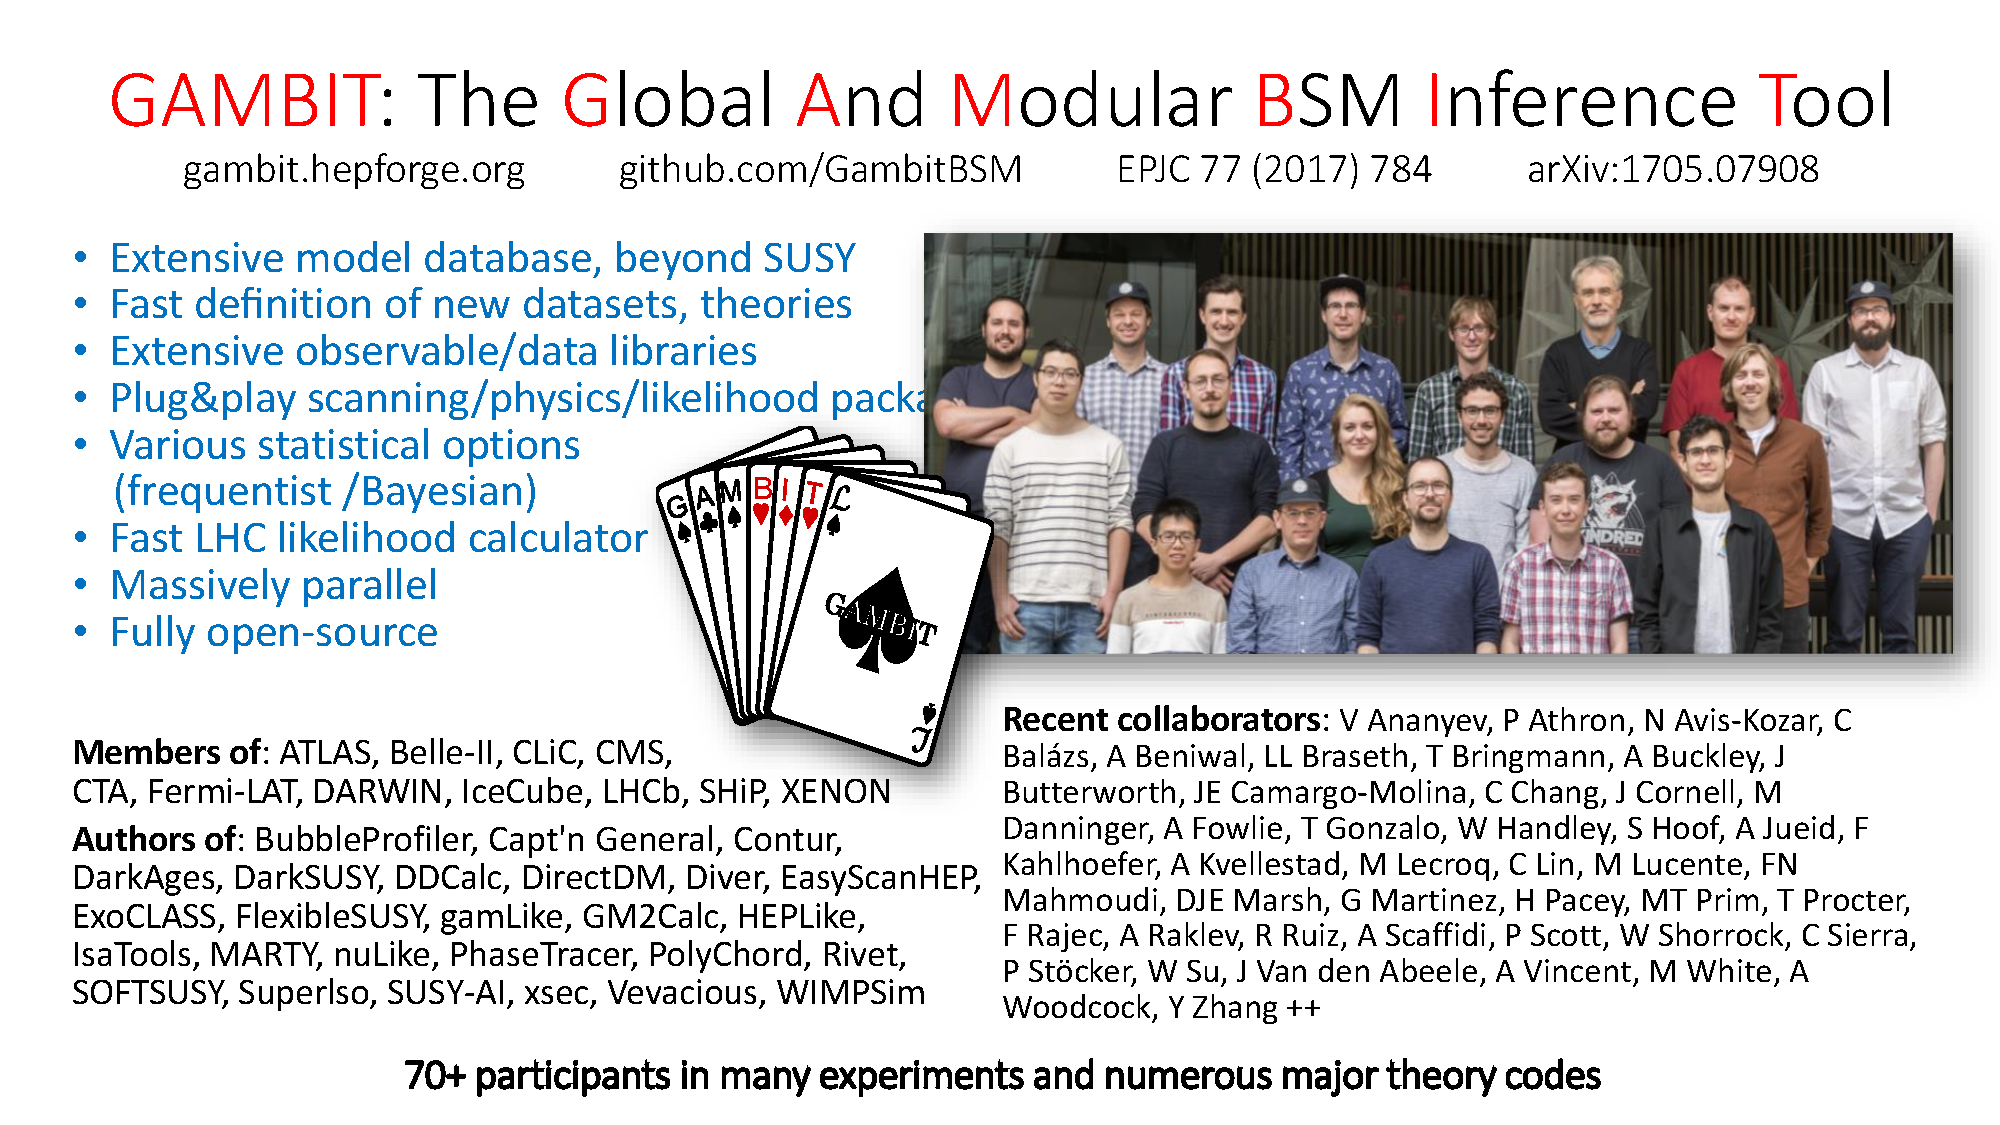
\includegraphics[width=\paperwidth]{gambit_ad_slide}}
    \begin{frame}[plain]
    \end{frame}
}

\end{document}
